\documentclass[a4paper,11pt,exos]{nsi} % COMPILE WITH DRAFT


\pagestyle{empty}
\begin{document}

%Exercice 1E12


\subsection*{NOM, Prénom : \dotfill} 

\classe{\premiere spé}
\titre{Ceinture verte 03}
\maketitle


\begin{exercice}[ : Trouver l'équation d'une parabole]
    Quelle est l'expression de la fonction polynomiale $f$ du second degré dont la parabole a pour sommet le point de coordonnées $(-2;-8)$ et passe par le point de coordonnées $(-3;-6)$ ?\\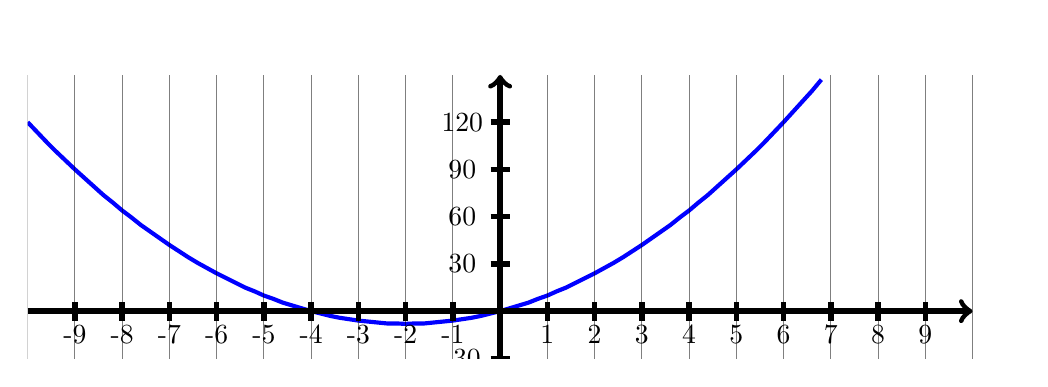
\begin{tikzpicture}[baseline,scale = 0.6]

        \tikzset{
          point/.style={
            thick,
            draw,
            cross out,
            inner sep=0pt,
            minimum width=5pt,
            minimum height=5pt,
          },
        }
        \clip (-10,-1) rectangle (11,6);
            
        \draw[color={blue},line width = 1.5] (-10,4)--(-9.8,3.79)--(-9.6,3.58)--(-9.4,3.38)--(-9.2,3.19)--(-9,3)--(-8.8,2.82)--(-8.6,2.64)--(-8.4,2.46)--(-8.2,2.3)--(-8,2.13)--(-7.8,1.98)--(-7.6,1.82)--(-7.4,1.68)--(-7.2,1.54)--(-7,1.4)--(-6.8,1.27)--(-6.6,1.14)--(-6.4,1.02)--(-6.2,0.91)--(-6,0.8)--(-5.8,0.7)--(-5.6,0.6)--(-5.4,0.5)--(-5.2,0.42)--(-5,0.33)--(-4.8,0.26)--(-4.6,0.18)--(-4.4,0.12)--(-4.2,0.06)--(-4,0)--(-3.8,-0.05)--(-3.6,-0.1)--(-3.4,-0.14)--(-3.2,-0.17)--(-3,-0.2)--(-2.8,-0.22)--(-2.6,-0.24)--(-2.4,-0.26)--(-2.2,-0.26)--(-2,-0.27)--(-1.8,-0.26)--(-1.6,-0.26)--(-1.4,-0.24)--(-1.2,-0.22)--(-1,-0.2)--(-0.8,-0.17)--(-0.6,-0.14)--(-0.4,-0.1)--(-0.2,-0.05)--(0,0)--(0.2,0.06)--(0.4,0.12)--(0.6,0.18)--(0.8,0.26)--(1,0.33)--(1.2,0.42)--(1.4,0.5)--(1.6,0.6)--(1.8,0.7)--(2,0.8)--(2.2,0.91)--(2.4,1.02)--(2.6,1.14)--(2.8,1.27)--(3,1.4)--(3.2,1.54)--(3.4,1.68)--(3.6,1.82)--(3.8,1.98)--(4,2.13)--(4.2,2.3)--(4.4,2.46)--(4.6,2.64)--(4.8,2.82)--(5,3)--(5.2,3.19)--(5.4,3.38)--(5.6,3.58)--(5.8,3.79)--(6,4)--(6.2,4.22)--(6.4,4.44)--(6.6,4.66)--(6.8,4.9);
        \draw[color={blue},line width = 1.5] ;
        \draw[color={blue},line width = 1.5] ;
        \draw[color={blue},line width = 1.5] ;
        \draw[color={blue},line width = 1.5] ;
        \draw[color={blue},line width = 1.5] ;
        \draw[color={blue},line width = 1.5] ;
        \draw[color={blue},line width = 1.5] ;
        \draw[color={blue},line width = 1.5] ;
        \draw[color={blue},line width = 1.5] ;
        \draw[color={blue},line width = 1.5] ;
        \draw[color={blue},line width = 1.5] ;
        \draw[color={blue},line width = 1.5] ;
        \draw[color={blue},line width = 1.5] ;
        \draw[color={blue},line width = 1.5] ;
        \draw[color={blue},line width = 1.5] ;
        \draw[color={blue},line width = 1.5] ;
        
        \draw[color ={black},line width = 2,->] (-10,0)--(10,0);
        \draw[color ={black},line width = 2,->] (0,-2)--(0,5);
        \draw[color ={black},opacity = 0.5] (1,-2)--(1,5);
        \draw[color ={black},opacity = 0.5] (2,-2)--(2,5);
        \draw[color ={black},opacity = 0.5] (3,-2)--(3,5);
        \draw[color ={black},opacity = 0.5] (4,-2)--(4,5);
        \draw[color ={black},opacity = 0.5] (5,-2)--(5,5);
        \draw[color ={black},opacity = 0.5] (6,-2)--(6,5);
        \draw[color ={black},opacity = 0.5] (7,-2)--(7,5);
        \draw[color ={black},opacity = 0.5] (8,-2)--(8,5);
        \draw[color ={black},opacity = 0.5] (9,-2)--(9,5);
        \draw[color ={black},opacity = 0.5] (10,-2)--(10,5);
        \draw[color ={black},opacity = 0.5] (-1,-2)--(-1,5);
        \draw[color ={black},opacity = 0.5] (-2,-2)--(-2,5);
        \draw[color ={black},opacity = 0.5] (-3,-2)--(-3,5);
        \draw[color ={black},opacity = 0.5] (-4,-2)--(-4,5);
        \draw[color ={black},opacity = 0.5] (-5,-2)--(-5,5);
        \draw[color ={black},opacity = 0.5] (-6,-2)--(-6,5);
        \draw[color ={black},opacity = 0.5] (-7,-2)--(-7,5);
        \draw[color ={black},opacity = 0.5] (-8,-2)--(-8,5);
        \draw[color ={black},opacity = 0.5] (-9,-2)--(-9,5);
        \draw[color ={black},opacity = 0.5] (-10,-2)--(-10,5);
        \draw[color ={black},line width = 2] (1,-0.2)--(1,0.2);
        \draw[color ={black},line width = 2] (2,-0.2)--(2,0.2);
        \draw[color ={black},line width = 2] (3,-0.2)--(3,0.2);
        \draw[color ={black},line width = 2] (4,-0.2)--(4,0.2);
        \draw[color ={black},line width = 2] (5,-0.2)--(5,0.2);
        \draw[color ={black},line width = 2] (6,-0.2)--(6,0.2);
        \draw[color ={black},line width = 2] (7,-0.2)--(7,0.2);
        \draw[color ={black},line width = 2] (8,-0.2)--(8,0.2);
        \draw[color ={black},line width = 2] (9,-0.2)--(9,0.2);
        \draw[color ={black},line width = 2] (-1,-0.2)--(-1,0.2);
        \draw[color ={black},line width = 2] (-2,-0.2)--(-2,0.2);
        \draw[color ={black},line width = 2] (-3,-0.2)--(-3,0.2);
        \draw[color ={black},line width = 2] (-4,-0.2)--(-4,0.2);
        \draw[color ={black},line width = 2] (-5,-0.2)--(-5,0.2);
        \draw[color ={black},line width = 2] (-6,-0.2)--(-6,0.2);
        \draw[color ={black},line width = 2] (-7,-0.2)--(-7,0.2);
        \draw[color ={black},line width = 2] (-8,-0.2)--(-8,0.2);
        \draw[color ={black},line width = 2] (-9,-0.2)--(-9,0.2);
        \draw[color ={black},line width = 2] (-0.2,1)--(0.2,1);
        \draw[color ={black},line width = 2] (-0.2,2)--(0.2,2);
        \draw[color ={black},line width = 2] (-0.2,3)--(0.2,3);
        \draw[color ={black},line width = 2] (-0.2,4)--(0.2,4);
        \draw[color ={black},line width = 2] (-0.2,-1)--(0.2,-1);
        \draw [color={black},fill opacity = 1] (1,-0.5) node[anchor = center,scale=1] {1};
        \draw [color={black},fill opacity = 1] (2,-0.5) node[anchor = center,scale=1] {2};
        \draw [color={black},fill opacity = 1] (3,-0.5) node[anchor = center,scale=1] {3};
        \draw [color={black},fill opacity = 1] (4,-0.5) node[anchor = center,scale=1] {4};
        \draw [color={black},fill opacity = 1] (5,-0.5) node[anchor = center,scale=1] {5};
        \draw [color={black},fill opacity = 1] (6,-0.5) node[anchor = center,scale=1] {6};
        \draw [color={black},fill opacity = 1] (7,-0.5) node[anchor = center,scale=1] {7};
        \draw [color={black},fill opacity = 1] (8,-0.5) node[anchor = center,scale=1] {8};
        \draw [color={black},fill opacity = 1] (9,-0.5) node[anchor = center,scale=1] {9};
        \draw [color={black},fill opacity = 1] (-1,-0.5) node[anchor = center,scale=1] {-1};
        \draw [color={black},fill opacity = 1] (-2,-0.5) node[anchor = center,scale=1] {-2};
        \draw [color={black},fill opacity = 1] (-3,-0.5) node[anchor = center,scale=1] {-3};
        \draw [color={black},fill opacity = 1] (-4,-0.5) node[anchor = center,scale=1] {-4};
        \draw [color={black},fill opacity = 1] (-5,-0.5) node[anchor = center,scale=1] {-5};
        \draw [color={black},fill opacity = 1] (-6,-0.5) node[anchor = center,scale=1] {-6};
        \draw [color={black},fill opacity = 1] (-7,-0.5) node[anchor = center,scale=1] {-7};
        \draw [color={black},fill opacity = 1] (-8,-0.5) node[anchor = center,scale=1] {-8};
        \draw [color={black},fill opacity = 1] (-9,-0.5) node[anchor = center,scale=1] {-9};
        \draw [color={black},fill opacity = 1] (-0.8,1) node[anchor = center,scale=1] {30};
        \draw [color={black},fill opacity = 1] (-0.8,2) node[anchor = center,scale=1] {60};
        \draw [color={black},fill opacity = 1] (-0.8,3) node[anchor = center,scale=1] {90};
        \draw [color={black},fill opacity = 1] (-0.8,4) node[anchor = center,scale=1] {120};
        \draw [color={black},fill opacity = 1] (-0.8,-1) node[anchor = center,scale=1] {-30};
    
    \end{tikzpicture}\\

\end{exercice}


\carreauxseyes{17.6}{13.6}
\end{document}